\section{Natural Language Based CLI Framework}

\begin{figure}[h]
    \begin{center} 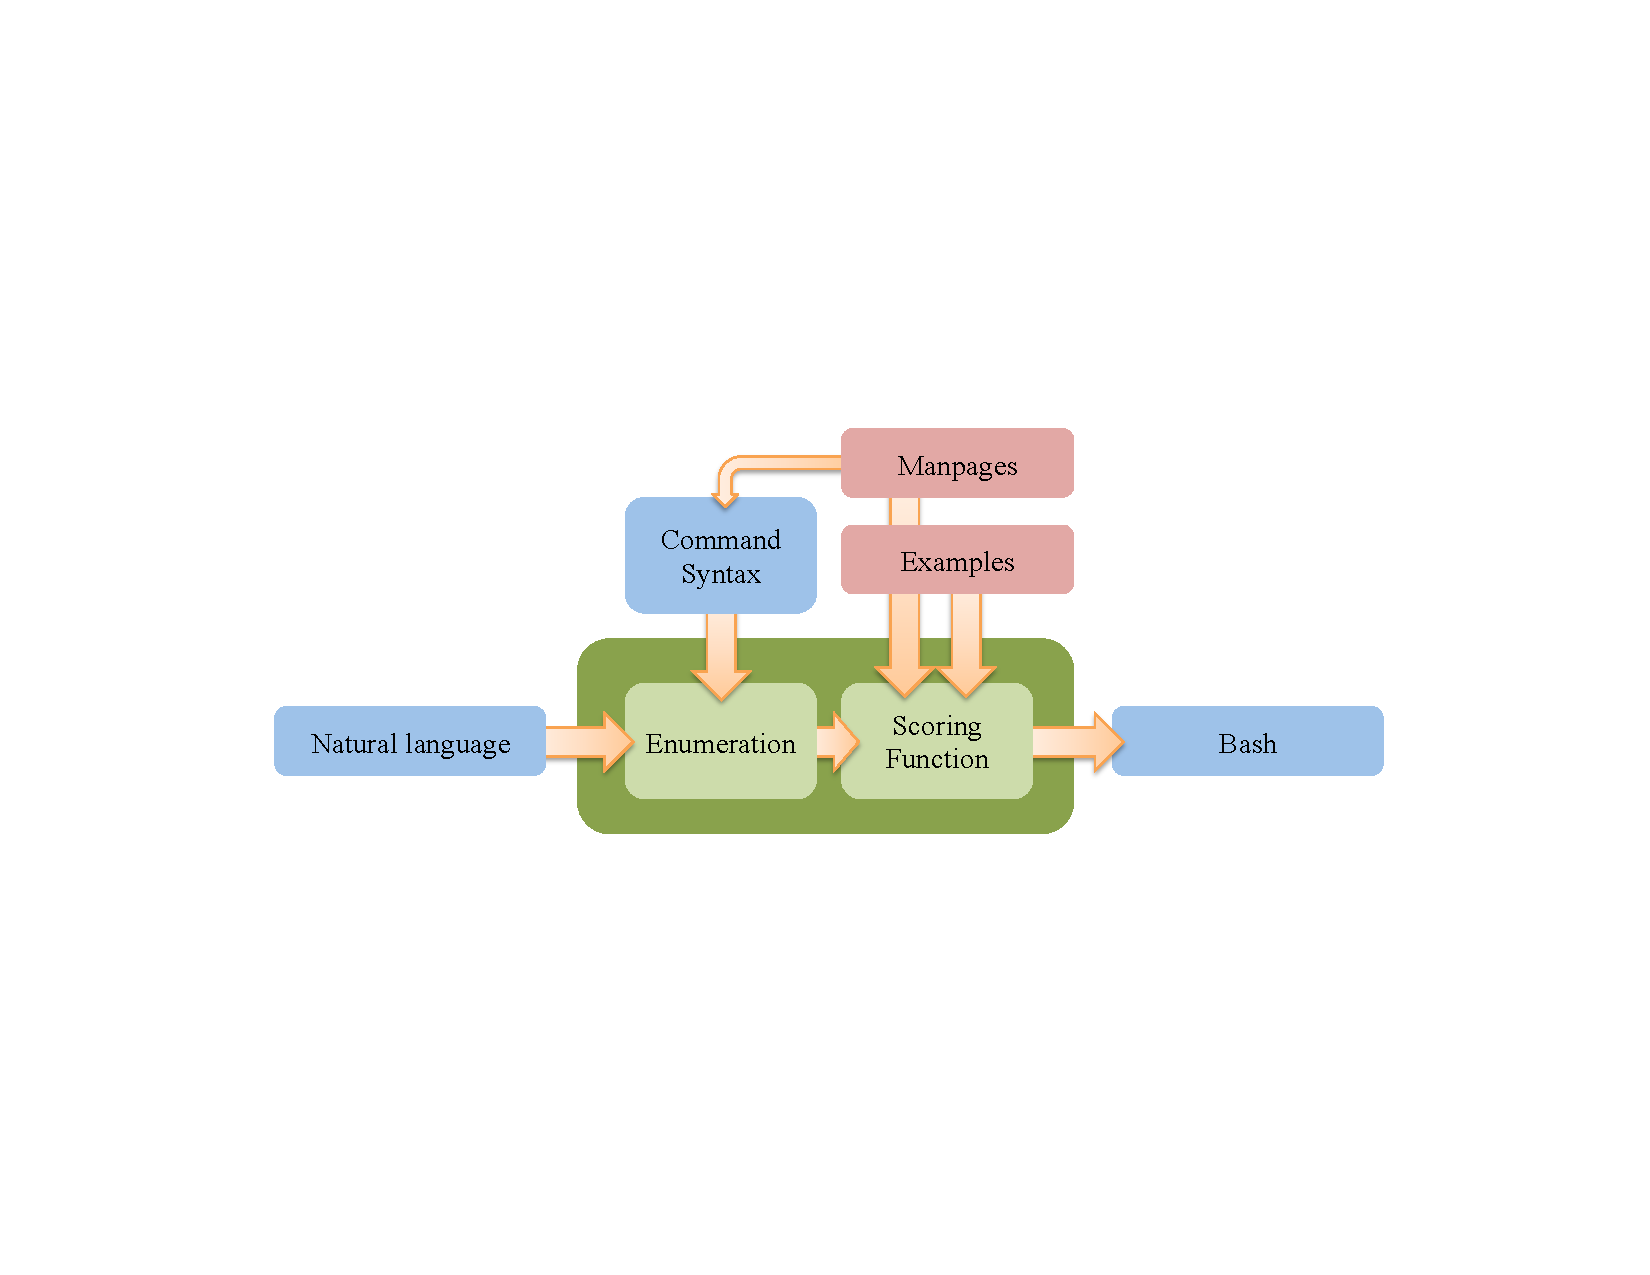
\includegraphics[width=4in]{architecture.pdf} \end{center}
    \caption{The overall architecture of our tool. Offline, the tool learns the
        valid syntax for common Bash commands using manpages. Both the manpages
        and a set of input-output examples are used to learn an appropriate
        scoring function. At runtime, the tool enumerates possible candidate
        programs using the learned syntax, scores them using the learned scoring
        function, and presents the top-ranked suggestions to the user.}
    \label{fig:arch}
\end{figure}

The natural language based command line interpreter we plan to develop consists of three key components: 1) an intermediate language  based on which Linux commands are generated and
% 2) a learning algorithm that can learn primitive commands of the intermediate language with provided man pages and 
2) a semantic parser that effectively maps the natural language commands issued by users to this intermediate representation. Especially, our initial pilot system is restricted to cover only file system operations, including file lookup, directory tree transformation, file content transformation, file property modifications. We restrict the domain in the hope that it can be expressed with tractable logic as well as to reduce the degree of ambiguity in the natural language command. Section~\ref{subsec:represent} introduces the formal language design and section~\ref{subsec:parser} introduces the approach to train the semantic parser.

\subsection{Language Design}
\label{subsec:represent}
An ideal intermediate language for the CLI programs should be 1) expressive enough so that it covers many interesting real world cases, 2) concise enough for the synthesizer to efficiently synthesize and 3) extensible, so that different people targeting different command line applications and use different sets of primitive commands.

Concretely, the syntax of the intermediate language design is presented below.

\begin{figure}
\[
\begin{array}{rlll}
\multicolumn{3}{l}{\textbf{Program}}\\
\mathit{p} & := & \mathit{value} \\
    &  & \mathit{cmd}~\overline{\mathit{flag}}~\overline{\mathit{arg}} & \textrm{(Program)}\\
    &  & \mathit{p} ~\| ~\mathit{p} & \textrm{(Pipelined program)}\\
\mathit{value} & := & \mathsf{date} ~|~ \mathsf{filename} ~|~ ... & \textrm{(Primitive values)}\\
\mathit{arg} & := & \epsilon ~|~ \mathit{value} ~|~ \mathit{hole} & \textrm{(Arguments)}\\
\mathit{cmd}^{*} & := & \mathsf{find} ~|~ \mathsf{grep} ~|~ ... & \textrm{(Commands)}\\
\mathit{flag}^{*} & := & \epsilon ~|~ -f ~|~ -h ~|~ ... & \textrm{(Flags)}\\
~\\
\multicolumn{3}{l}{\textbf{Command Signature}}\\
\mathit{sig} & := & \mathsf{name}~\mathit{option}:\tau & \textrm{(Command signature)}\\
\mathit{option} &:= & \mathsf{flagname} & \textrm{(Command option)}\\
                &   & \mathsf{argname}[\tau]\\
                &   & \mathit{option}~\mathbf{or}~\mathit{option}\\
                &   & [ \mathit{option} ]\\
~\\
\multicolumn{3}{l}{\textbf{Rules}}\\
\mathit{rule}^{*} &:=& \mathsf{find}~f[\mathsf{File}] : \mathsf{File}\\
                  &  & \mathit{date}~\mathit{-d} : \mathsf{void}\\
                  &  & \mathit{date}~\mathit{-u} : \mathsf{Date}\\
                  &  & ...\\
~\\
\multicolumn{3}{l}{\textbf{Types}}\\
\tau_0 & := & \mathsf{void} ~|~ \mathsf{File} & \textrm{(Primitive types)}\\
       &     & |~ \mathsf{Date} ~|~ \mathsf{Permission} ~|~ \mathsf{Size} ~|~ ... \\
\tau & := & \tau_0 ~|~ \tau_0\rightarrow \tau_0 & \textrm{(Type)}
\end{array}
\]
\caption{Intermediate Language}
\label{fig:lang}
\end{figure}


The first part of our language is the program syntax (labeled as \textbf{Program}), defines how a program can be formed: a CLI program can be 1) refer to a value, 2) call a primitive command, and 3) pipelining two programs and passing the result of the first program as the argument of the second program.

The rest of the language are designed to help check well-formedness of a given CLI program. The command signature defines how a rule can be written, the rules (\textbf{Rule}) defines which primitive programs are valid. Then, with the help of the types in our program, we can check the type of a program $p$ to ensure that a command line program is well-formed.

Since the number of basic Linux commands and options is large even in domain-specific scenarios, it is difficult for a human designer to hand-code all of the generation rules. We plan to semi-automate this step by adding information extracted from the Linux man pages\footnote{\url{http://linux.die.net/man/}} and make the language extensible. Concretely, we shall parse the man page to generate primitive commands, flags and checking rules for each command (all non-terminals labeled with * in Figure~\ref{fig:lang} will be automatically learned from man page). And with this language design, users can extend the basic language by providing man pages.

\subsection{Natural Language Command Interpreter}
\label{subsec:parser}
We train the natural language command interpreter using the Linux man pages, in addition to a small set of natural language and command line program pairs. The motivation of adopting man pages as one resource of the training data lies in the fact that gathering sufficient number of of natural language to command line program pairs is expensive. The large volume of Stack Overflow conversations are noisy and only a handful of high-quality training pairs can be confidently extracted. On the other hand, the Linux man pages are well formatted and contains rich natural language text that explains the usage of each command template and its possible arguments. We propose to use the command-explanation pairs extracted from man pages as additional signals to guide the search for high score rankings, thereby remedies the lack of example training pairs.

We use a linear feature function to score the natural language command to logical representation mappings. The following features are used:
\begin{itemize}\itemsep-1pt
	\item association of key words/phrases to partial expressions
	\item association between partial expressions (e.g. how often do they combined in valid commands)
	\item similarity of key words/phrases in the command to the man page explanation text of a partial expression
	\item complexity of the logical formulas and the commands generated from them.
\end{itemize}
We use the structured perceptron algorithm to learn weights of the scoring function from the example pairs. In each training iteration, we search for the top ranked logical form and update the weights based on its similarity to the ground truth logical form.
% We planned to extend learning into an interactive setting once the basic framework is developed.